\documentclass[aspectratio=169]{beamer}

%\documentclass[handout]{beamer}
%% To make 4 per page
%\usepackage{pgfpages}
%\mode<handout>{\setbeamercolor{background canvas}{bg=white}}
%\pgfpagesuselayout{4 on 1}[letterpaper,landscape]%,border shrink=5mm]

\usetheme{default}
\usepackage{bm}
\usepackage{colortbl}

\usepackage{amsmath,amssymb,amsthm}
%\usepackage{subfigure}


% Fields and the like
\def\IC{\mathbb{C}}
\def\IF{\mathbb{F}}
\def\II{\mathbb{I}}
\def\IM{\mathbb{M}}
\def\IN{\mathbb{N}}
\def\IP{\mathbb{P}}
\def\IR{\mathbb{R}}
\def\IZ{\mathbb{Z}}

% Bold lowercase
\def\ba{\mathbf{a}}
\def\bb{\mathbf{b}}
\def\bc{\mathbf{c}}
\def\bd{\mathbf{d}}
\def\be{\mathbf{e}}
\def\bf{\mathbf{f}}
\def\bh{\mathbf{h}}
\def\bi{\mathbf{i}}
\def\bj{\mathbf{j}}
\def\bk{\mathbf{k}}
\def\bn{\mathbf{n}}
\def\bp{\mathbf{p}}
\def\br{\mathbf{r}}
\def\bs{\mathbf{s}}
\def\bu{\mathbf{u}}
\def\bv{\mathbf{v}}
\def\bw{\mathbf{w}}
\def\bx{\mathbf{x}}
\def\by{\mathbf{y}}
\def\bz{\mathbf{z}}

% Bold capitals
\def\bB{\mathbf{B}}
\def\bD{\mathbf{D}}
\def\bF{\mathbf{F}}
\def\bG{\mathbf{G}}
\def\bI{\mathbf{I}}
\def\bL{\mathbf{L}}
\def\bN{\mathbf{N}}
\def\bR{\mathbf{R}}
\def\bS{\mathbf{S}}
\def\bT{\mathbf{T}}
\def\bX{\mathbf{X}}

% Bold numbers
\def\b0{\mathbf{0}}

% Bold greek
\bmdefine{\bmu}{\bm{\mu}}
\def\bphi{\bm{\phi}}
\def\bvarphi{\bm{\varphi}}

% Bold red sentence
\def\boldred#1{{\color{red}\textbf{#1}}}
\def\defword#1{{\color{orange}\textbf{#1}}}

% Caligraphic letters
\def\A{\mathcal{A}}
\def\B{\mathcal{B}}
\def\C{\mathcal{C}}
\def\D{\mathcal{D}}
\def\E{\mathcal{E}}
\def\F{\mathcal{F}}
\def\G{\mathcal{G}}
\def\I{\mathcal{I}}
\def\L{\mathcal{L}}
\def\M{\mathcal{M}}
\def\P{\mathcal{P}}
\def\R{\mathcal{R}}
\def\S{\mathcal{S}}
\def\T{\mathcal{T}}
\def\U{\mathcal{U}}
\def\V{\mathcal{V}}

% tt font for code
\def\code#1{{\tt #1}}

% Operators and special symbols
\def\nbOne{{\mathchoice {\rm 1\mskip-4mu l} {\rm 1\mskip-4mu l}
{\rm 1\mskip-4.5mu l} {\rm 1\mskip-5mu l}}}
\def\cov{\ensuremath{\mathsf{cov}}}
\def\Var{\ensuremath{\mathsf{Var}\ }}
\def\Im{\textrm{Im}\;}
\def\Re{\textrm{Re}\;}
\def\det{\ensuremath{\mathsf{det}}}
\def\diag{\ensuremath{\mathsf{diag}}}
\def\nullspace{\ensuremath{\mathsf{null}}}
\def\nullity{\ensuremath{\mathsf{nullity}}}
\def\rank{\ensuremath{\mathsf{rank}}}
\def\range{\ensuremath{\mathsf{range}}}
\def\sgn{\ensuremath{\mathsf{sgn}}}
\def\Span{\ensuremath{\mathsf{span}}}
\def\tr{\ensuremath{\mathsf{tr}}}
\def\imply{$\Rightarrow$}
\def\restrictTo#1#2{\left.#1\right|_{#2}}
\newcommand{\parallelsum}{\mathbin{\!/\mkern-5mu/\!}}

% The beamer bullet (in base colour)
\def\bbullet{\leavevmode\usebeamertemplate{itemize item}\ }

% Theorems and the like
\newtheorem{proposition}[theorem]{Proposition}
\newtheorem{property}[theorem]{Property}
\newtheorem{importantproperty}[theorem]{Property}
\newtheorem{importanttheorem}[theorem]{Theorem}
%\newtheorem{lemma}[theorem]{Lemma}
%
%\usecolortheme{orchid}
\setbeamertemplate{theorems}[numbered]
%\usecolortheme{orchid}
%\setbeamertemplate{theorems}[ams style]
%\setbeamertemplate{theorems}[numbered]

%% Listings
\usepackage{listings}
\definecolor{mygreen}{rgb}{0,0.6,0}
\definecolor{mygray}{rgb}{0.5,0.5,0.5}
\definecolor{mymauve}{rgb}{0.58,0,0.82}
\definecolor{mygold}{rgb}{1,0.843,0}
\definecolor{myblue}{rgb}{0.537,0.812,0.941}

\definecolor{lgreen}{rgb}{0.6,0.9,.6}
\definecolor{lred}{rgb}{1,0.5,.5}

\lstloadlanguages{R}
\lstset{ %
  language=R,
  backgroundcolor=\color{black!95},   % choose the background color
  basicstyle=\footnotesize\ttfamily,        % size of fonts used for the code
  breaklines=true,                 % automatic line breaking only at whitespace
  captionpos=b,                    % sets the caption-position to bottom
  commentstyle=\color{mygreen},    % comment style
  escapeinside={\%*}{*)},          % if you want to add LaTeX within your code
  keywordstyle=\color{myblue},       % keyword style
  stringstyle=\color{mygold},     % string literal style
  keepspaces=true,
  columns=fullflexible,
  tabsize=4,
}
% Could also do (in lstset)
% basicstyle==\fontfamily{pcr}\footnotesize


% Get rid of navigation stuff
\setbeamertemplate{navigation symbols}{}

% Set footline/header line
\setbeamertemplate{footline}
{%
\quad p. \insertpagenumber \quad--\quad \insertsection\vskip2pt
}
% \setbeamertemplate{headline}
% {%
% \quad\insertsection\hfill p. \insertpagenumber\quad\mbox{}\vskip2pt
% }


\makeatletter
\newlength\beamerleftmargin
\setlength\beamerleftmargin{\Gm@lmargin}
\makeatother

%%%%%%% 
%% Definitions in yellow boxes
\usepackage{etoolbox}
\setbeamercolor{block title}{use=structure,fg=structure.fg,bg=structure.fg!05!bg}
\setbeamercolor{block body}{parent=normal text,use=block title,bg=block title.bg!20!bg}

\BeforeBeginEnvironment{definition}{%
	\setbeamercolor{block title}{fg=black,bg=yellow!20!white}
	\setbeamercolor{block body}{fg=black, bg=yellow!05!white}
}
\AfterEndEnvironment{definition}{
	\setbeamercolor{block title}{use=structure,fg=structure.fg,bg=structure.fg!20!bg}
	\setbeamercolor{block body}{parent=normal text,use=block title,bg=block title.bg!50!bg, fg=black}
}
\BeforeBeginEnvironment{importanttheorem}{%
	\setbeamercolor{block title}{fg=black,bg=red!20!white}
	\setbeamercolor{block body}{fg=black, bg=red!05!white}
}
\AfterEndEnvironment{importanttheorem}{
	\setbeamercolor{block title}{use=structure,fg=structure.fg,bg=structure.fg!20!bg}
	\setbeamercolor{block body}{parent=normal text,use=block title,bg=block title.bg!50!bg, fg=black}
}
\BeforeBeginEnvironment{theorem}{%
	\setbeamercolor{block title}{fg=white,bg=red!30!black}
	\setbeamercolor{block body}{fg=white, bg=red!10!black}
}
\AfterEndEnvironment{theorem}{
	\setbeamercolor{block title}{use=structure,fg=structure.fg,bg=structure.fg!20!bg}
	\setbeamercolor{block body}{parent=normal text,use=block title,bg=block title.bg!50!bg, fg=black}
}
\BeforeBeginEnvironment{importantproperty}{%
	\setbeamercolor{block title}{fg=black,bg=red!50!white}
	\setbeamercolor{block body}{fg=black, bg=red!30!white}
}
\AfterEndEnvironment{importantproperty}{
	\setbeamercolor{block title}{use=structure,fg=structure.fg,bg=structure.fg!20!bg}
	\setbeamercolor{block body}{parent=normal text,use=block title,bg=block title.bg!50!bg, fg=black}
}


%%%%%%%%%%%%%%%%%
\usepackage{tikz}
\usetikzlibrary{shapes,arrows}
\usetikzlibrary{positioning}
\usetikzlibrary{shapes.symbols,shapes.callouts,patterns}
\usetikzlibrary{calc,fit}
\usetikzlibrary{backgrounds}
\usetikzlibrary{decorations.pathmorphing,fit,petri}
\usetikzlibrary{automata}
\usetikzlibrary{fadings}
\usetikzlibrary{patterns,hobby}

\usepackage{pgfplots}
\pgfplotsset{compat=1.6}
\pgfplotsset{ticks=none}

\usetikzlibrary{decorations.markings}
\usetikzlibrary{arrows.meta}
\tikzset{>=stealth}

\tikzstyle{cloud} = [draw, 
ellipse,
fill=red!20, 
node distance=0.87cm,
minimum height=2em]
\tikzstyle{line} = [draw, 
-latex', 
color=yellow]


% Beginning of a section
% \AtBeginSection[]{
% 	{
% 		\setbeamercolor{background canvas}{bg=orange!10}
% 		\begin{frame}[noframenumbering,plain]
% 			\framesubtitle{\nameofthepart Chapter \insertromanpartnumber \ -- \iteminsert{\insertpart}}
% 			\tableofcontents[currentsection,currentsubsection]
% 		\end{frame}
% 	\addtocounter{page}{-1}
% 	%\addtocounter{framenumber}{-1} 
% 	}
% }


%%% SLIDES COLOURING

%\usecolortheme{owl}

\setbeamerfont{frametitle}{series=\bfseries}
\setbeamercolor{frametitle}{fg=black!05,bg=black}

\setbeamerfont{framesubtitle}{size=\normalfont\tiny}
\setbeamercolor{framesubtitle}{fg=black!05}

\setbeamercolor{background canvas}{bg=black}
\setbeamercolor{normal text}{fg=black!10}



\definecolor{bottomcolour}{rgb}{0.32,0.3,0.38}
\definecolor{middlecolour}{rgb}{0.08,0.08,0.16}
\definecolor{mycolor}{rgb}{0.4,0.4, 0.4}
% Beginning of a section
\AtBeginSection[]{
	{
		%\setbeamercolor{background canvas}[vertical shading][top=bottomcolour, middle=middlecolour, bottom=black]
		\setbeamertemplate{background canvas}[vertical shading][bottom=bottomcolour,top=black!20]
    % \setbeamertemplate{background canvas}{
    %   \begin{tikzpicture}%[remember picture,overlay]
    %     \shade[top color=yellow!75!green!33,
    %     bottom color=blue!66!green!33,
    %     middle color=blue!6!green!33]
    %   \end{tikzpicture}
    % }
    \begin{frame}[noframenumbering,plain]
			\framesubtitle{\nameofthepart Chapter \insertromanpartnumber \ -- \iteminsert{\insertpart}}
			\tableofcontents[currentsection,currentsubsection]
		\end{frame}
	\addtocounter{page}{-1}
	}
}
% Beginning of a section
\AtBeginSubsection[]{
	{
		%\setbeamercolor{background canvas}[vertical shading][top=bottomcolour, middle=middlecolour, bottom=black]
		%\setbeamertemplate{background canvas}[vertical shading][bottom=bottomcolour,top=black!20]
    \setbeamertemplate{background canvas}{
      \begin{tikzpicture}%[remember picture,overlay]
        \shade[top color=yellow!75!green!33,
        bottom color=blue!66!green!33,
        middle color=blue!6!green!33]
      \end{tikzpicture}
    }
    \begin{frame}[noframenumbering,plain]
			\framesubtitle{\nameofthepart Chapter \insertromanpartnumber \ -- \iteminsert{\insertpart}}
			\tableofcontents[currentsection,currentsubsection]
		\end{frame}
	\addtocounter{page}{-1}
	}
}

% Colours for special pages
\def\extraContent{yellow!20}

%% Allow to change slide colour
%% From: https://tex.stackexchange.com/questions/8043/change-the-background-color-of-a-frame-in-beamer
\defbeamertemplate*{background canvas}{mydefault}{%
  \ifbeamercolorempty[bg]{background canvas}{}{\color{bg}\vrule width\paperwidth height\paperheight}% copied beamer default here
}
\defbeamertemplate*{background canvas}{bg}{%
  \color{lightgray!20}\vrule width\paperwidth height\paperheight% added bg color
}
\BeforeBeginEnvironment{frame}{%
  \setbeamertemplate{background canvas}[mydefault]%
}
\makeatletter
\define@key{beamerframe}{bg}[true]{%
  \setbeamertemplate{background canvas}[bg]%
}
\makeatother
% Use with
%\begin{frame}
% \frametitle{Normal}
%\end{frame} 
%\begin{frame}[bg]
% \frametitle{With bg}
%\end{frame}


%% Vertical alignment on pages
%% From: https://tex.stackexchange.com/questions/148365/how-do-i-ask-beamer-to-exactly-fill-up-a-slide
%% Turn on with
%% \stretchon
%% (outside slide), and off with
%% \stretchoff
% \def\itemsymbol{$\blacktriangleright$}
% \let\svpar\par
% \let\svitemize\itemize
% \let\svenditemize\enditemize
% \let\svitem\item
% \let\svcenter\center
% \let\svendcenter\endcenter
% \let\svcolumn\column
% \let\svendcolumn\endcolumn
% \def\newitem{\renewcommand\item[1][\itemsymbol]{\vfill\svitem[##1]}}%
% \def\newpar{\def\par{\svpar\vfill}}%
% \newcommand\stretchon{%
%   \newpar%
%   \renewcommand\item[1][\itemsymbol]{\svitem[##1]\newitem}%
%   \renewenvironment{itemize}%
%     {\svitemize}{\svenditemize\newpar\par}%
%   \renewenvironment{center}%
%     {\svcenter\newpar}{\svendcenter\newpar}%
%   \renewenvironment{column}[2]%
%     {\svcolumn{##1}\setlength{\parskip}{\columnskip}##2}%
%     {\svendcolumn\vspace{\columnskip}}%
% }
% \newcommand\stretchoff{%
%   \let\par\svpar%
%   \let\item\svitem%
%   \let\itemize\svitemize%
%   \let\enditemize\svenditemize%
%   \let\center\svcenter%
%   \let\endcenter\svendcenter%
%   \let\column\svcolumn%
%   \let\endcolumn\svendcolumn%
% }
% \newlength\columnskip
% \columnskip 0pt



\title{Environmentally Transmitted Pathogens}
\subtitle{Models -- Part deux :)}
\author{Julien Arino}
\date{January 2023}


\begin{document}
%\stretchon

% The title page
\begin{frame}[noframenumbering,plain]
  \titlepage
\end{frame}
\addtocounter{page}{-1}

%%%%%%%%%%%%%%%%%%%%
%%%%%%%%%%%%%%%%%%%%
%%%%%%%%%%%%%%%%%%%%
%%%%%%%%%%%%%%%%%%%%
\section{Some considerations about numerics}
%%%%%%%%%%%%%%%%%%%%
%%%%%%%%%%%%%%%%%%%%
\subsection{The tetanus model of Cvjetanovi\'c}

\begin{frame}
  \begin{center}
    \def\vertskip{*-2}
    \def\horzskip{*2}
    \begin{tikzpicture}[scale=0.75, transform shape]
      \node [rectangle, fill=gray!10, text=black] at (-2\horzskip,0\vertskip) (S_nb) {Newborn};
      \node [rectangle, fill=gray!10, text=black] at (2\horzskip,0\vertskip) (S) {Susceptible population};
      \node [rectangle, fill=gray!10, text=black] at (-2\horzskip,1\vertskip) (L_nb) {Incubating newborn};
      \node [rectangle, fill=gray!10, text=black] at (2\horzskip,1\vertskip) (L) {Incubating population};
      \node [rectangle, fill=gray!10, text=black] at (-2\horzskip,2\vertskip) (I_nb) {Sick newborn};
      \node [rectangle, fill=gray!10, text=black] at (2\horzskip,2\vertskip) (I) {Sick population};
      \node [rectangle, fill=gray!10, text=black] at (0\horzskip,3\vertskip) (D) {Tetanus deaths};
      \node [rectangle, fill=gray!10, text=black] at (0\horzskip,4\vertskip) (R) {Active immunity 10 years};
      \node [rectangle, fill=gray!10, text=black] at (0\horzskip,5\vertskip) (R_p) {Passive immunity 6 months};
      %% Flows
      \path [line, very thick] (S_nb) to node [midway, above] (TextNode) {} (S);
      \path [line, very thick] (S_nb) to node [midway, above] (TextNode) {} (L_nb);
      \path [line, very thick] (L_nb) to node [midway, above] (TextNode) {} (I_nb);
      \path [line, very thick] (I_nb) to node [midway, above] (TextNode) {} (D);
      \path [line, very thick] (I_nb) to node [midway, above] (TextNode) {} (R);
      \path [line, very thick, bend right=60] (S_nb.west) to node [midway, above] (TextNode) {} (R_p.west);
      \path [line, very thick] (I_nb) to node [midway, above] (TextNode) {} (S.-170);
      \path [line, very thick] (I_nb) to node [midway, above] (TextNode) {} (R);
      \path [line, very thick] (I_nb) to node [midway, above] (TextNode) {} (D);
      \path [line, very thick] (S) to node [midway, above] (TextNode) {} (L);
      \path [line, very thick] (L) to node [midway, above] (TextNode) {} (I);
      \path [line, very thick, bend left=75] (I) to node [midway, above] (TextNode) {} (S);
      \path [line, very thick] (I) to node [midway, above] (TextNode) {} (R);
      \path [line, very thick] (I) to node [midway, above] (TextNode) {} (D);
      \path [line, very thick, bend right=60] (R.east) to node [midway, above] (TextNode) {} (S.-10);      
      \path [line, very thick, bend right=60, anchor=east] (R_p.east) to node [midway, above] (TextNode) {} (S.east);      
    \end{tikzpicture}    
  \end{center}  
\end{frame}

\begin{frame}{Flow diagram (demography not shown)}
  \begin{center}
    \def\vertskip{*-1.75}
    \def\horzskip{*1}
    \begin{tikzpicture}[scale=0.8, transform shape]
      \node [rectangle, fill=gray!10, text=black] at (-2\horzskip,0\vertskip) (S_nb) {$S_b$};
      \node [rectangle, fill=gray!10, text=black] at (2\horzskip,0\vertskip) (S) {$S$};
      \node [rectangle, fill=gray!10, text=black] at (-2\horzskip,1\vertskip) (L_nb) {$L_b$};
      \node [rectangle, fill=gray!10, text=black] at (2\horzskip,1\vertskip) (L) {$L$};
      \node [rectangle, fill=gray!10, text=black] at (-2\horzskip,2\vertskip) (I_nb) {$I_b$};
      \node [rectangle, fill=gray!10, text=black] at (2\horzskip,2\vertskip) (I) {$I$};
      \node [rectangle, fill=gray!10, text=black] at (0\horzskip,3\vertskip) (D) {$D$};
      \node [rectangle, fill=gray!10, text=black] at (0\horzskip,4\vertskip) (R) {$R$};
      \node [rectangle, fill=gray!10, text=black] at (0\horzskip,4.9\vertskip) (R_p) {$R_b$};
      %% Flows (newborn)
      \path [line, very thick] (S_nb) to node [midway,above] (TextNode) {$b(1-\lambda_b)(T-R)$} (S);
      \path [line, very thick] (S_nb) to node [midway,right] (TextNode) {$\lambda_bb(T-R)$} (L_nb);
      \path [line, very thick] (L_nb) to node [midway,above,sloped] (TextNode) {$\varepsilon_bL_b$} (I_nb);
      \path [line, very thick] (I_nb) to node [midway,above,sloped] (TextNode) {$\pi_{I_bD}\gamma_bI_b$} (D);
      \path [line, very thick] (I_nb) to node [midway,below,sloped] (TextNode) {$\pi_{I_bR}\gamma_bI_b$} (R);
      \path [line, very thick, bend right=60] (S_nb.west) to node [midway,above] (TextNode) {$bR$} (R_p.west);
      \path [line, very thick] (I_nb) to node [sloped,pos=0.4,above] (TextNode) {$\pi_{I_bS}\gamma_bI_b$} (S.-170);
      \path [line, very thick, bend right=60, anchor=east] (R_p.east) to node [midway,below,sloped] (TextNode) {$\nu_bI_b$} (S.east);      
      %% Flows (others)
      \path [line, very thick] (S) to node [midway,right] (TextNode) {$\lambda S$} (L);
      \path [line, very thick] (L) to node [midway,above,sloped] (TextNode) {$\varepsilon L$} (I);
      \path [line, very thick, bend left=55] (I) to node [sloped,midway,below] (TextNode) {$\tau_{IS}\gamma I$} (S.south west);
      \path [line, very thick] (I) to node [midway,below,sloped] (TextNode) {$\pi_{IR}\gamma I$} (R);
      \path [line, very thick] (I) to node [midway,above,sloped] (TextNode) {$\pi_{ID}\gamma I$} (D);
      \path [line, very thick, bend right=60] (R.east) to node [midway,below,sloped] (TextNode) {$\nu R$} (S.-10);
    \end{tikzpicture}    
  \end{center}  
\end{frame}

\begin{frame}{The discrete-time tetanus model (notation mine)}
  \begin{subequations}
    \begin{align}
      \Delta S_b &= bT \\
      \Delta S &= b(1-\lambda_b)(T-R)+\nu R+\nu_bI_b+\nu I+\pi_{I_bS}\gamma_bI_b+\pi_{IS}\gamma I \\ 
      &\quad -(\lambda+d-\delta_T)S \nonumber \\
      \Delta L_b &= \lambda_bb(T-R)-(\varepsilon_b+d-\delta_T)L_b \\
      \Delta L &= \lambda S-(\varepsilon+d-\delta_T)L \\
      \Delta I_b &= \varepsilon_bL_b-(\gamma_b+d-\delta_T)I \\
      \Delta I &= \varepsilon L-(\gamma+d-\delta_T)I \\
      \Delta R &= \pi_{I_bR}\gamma_bI_b+\pi_{IR}\gamma I-(\nu+d-\delta_T)R \\
      \Delta R_b &= bR-(\nu_b+d-\delta_T)R_b\\
      \Delta D &= \pi_{I_bD}\gamma_bI_b+\pi_{ID}\gamma I
    \end{align}
    where
    \begin{equation}
      T = S+L_b+L+I_b+I+R+R_b
      \quad\text{and}\quad
      \delta_T = \frac{\Delta D}{T}
    \end{equation}
  \end{subequations}
\end{frame}

\begin{frame}{Parameter assumptions -- Tetanus}
  \begin{itemize}
    \item \textbf{Incubation period --} Mean duration 6 days for newborn and 8 days for general population $\Rightarrow$ daily rate of exit $\varepsilon_b=0.1667$ and $\varepsilon=0.125$
    \item \textbf{Period of sickness --} Mean duration 3 days for newborn and 14 days for general population $\Rightarrow$ daily rate of exit $\gamma_b=0.3333$ per sick newborn and $\gamma=0.0714$ for sick general in general population
    \item \textbf{Mortality from tetanus --} Untreated tetanus cases, fatality rate 90\% for newborn $S_b$ and 40\% for general population. Treated: 80\% for newborn and 30\% general population
    \item \textbf{Immunity --} Tetanus cases do not lead to immunity to reinfection. But as a general rule, recovered people are vaccinated. Convalescents and general population effectively immunised by complete course of vaccination go to $R$ for average 10 years, daily rate of exit is $\nu=0.000274$ per person.
    \item \textbf{Immunity of newborns --} Newborn to women vaccinated during pregnancy are temporarily protected by maternal antibodies and pass through $R_b$ for a mean duration of 6 months. Daily rate of exit $\nu_b=0.005479$ per immunised newborn
  \end{itemize}
\end{frame}

\begin{frame}{Deciding on infection outcome -- $\pi$}
  Parameters $\pi$ are proportion of individuals who follow a certain route post-infection
  \vfill
  \begin{itemize}
    \item $\pi_{I_b\bullet}$ proportion of infected newborn who
    \begin{itemize}
      \item $\pi_{I_bS}$ recover without immunity
      \item $\pi_{I_bR}$ recover with immunity
      \item $\pi_{I_bD}$ die (0.9)
    \end{itemize}
    $\pi_{I_bS}+\pi_{I_bR}+\pi_{I_bD}=1$
    \vfill
    \item $\pi_{I\bullet}$ proportion of infected who
    \begin{itemize}
      \item $\pi_{IS}$ recover without immunity
      \item $\pi_{IR}$ recover with immunity
      \item $\pi_{ID}$ die (0.4)
    \end{itemize}
    $\pi_{IS}+\pi_{IR}+\pi_{ID}=1$
  \end{itemize}
\end{frame}

\begin{frame}{Parameter assumptions -- Demography}
  Live birth rate 35 per 1,000 population and annual crude death rate 15 per 1,000 population (annual rate of growth 2\%) $\Rightarrow$ daily birth and death rates $b=0.00009889$ and $d=0.0000411$ per person, respectively
\end{frame}

\begin{frame}{Parameter assumptions -- Force of infection}
  No H2H transmission $\Rightarrow$ incidence proportional to number of susceptible individuals and force of infection, which quantifies combined effect of all variables involved in infection process:
  \begin{itemize}
    \item degree of soil contamination with \emph{Clostridium tetani}
    \item climate
    \item frequency of lesions
    \item proportion of rural population
    \item socioeconomic conditions
    \item level of medical care for the wounded and during deliveries
  \end{itemize}
\end{frame}

\begin{frame}
  Force of infection acting on newborn ($\lambda_b$) and susceptible population ($\lambda$) fixed at 3 different levels adequate for reproducing the following stable annual incidence rates of tetanus cases in the community
  \begin{itemize}
    \item For newborn, 200 cases, 400 cases and 600 cases per 100,000 newborn
    \item For general population (without newborn), 9, 18 and 27 cases
  \end{itemize}
\end{frame}

\begin{frame}{A crash course on discrete-time systems}
  We have seen systems of ordinary differential equations (ODE) of the form 
  \[
    \frac{d}{dt}x(t)=f(x(t))
  \]
  often written omitting dependence on $t$, i.e.,
  \begin{equation}\label{eq:ODE}
    x' = f(x)
  \end{equation}
  where $x\in\IR^n$ and $f:\IR^n\to\IR^n$. The system is considered together with an initial condition $x(t_0)=x_0\in\IR^n$.
  \vfill
  The \textbf{independent} variable $t\in\IR$
\end{frame}

\begin{frame}
  A discrete-time system takes the form
  \begin{equation}\label{eq:DTS}
    x(t+\Delta t) = f(x(t))
  \end{equation}
  where $x(t)\in\IR^n$ and $f:\IR^n\to\IR^n$
  \vfill
  In a discrete-time system, $t$ is discrete and can be assumed to be in $\IZ$ or $\IN$ (in practice, before ``recasting'', it is in $\mathbb{Q}$), we often write $x(t+1)=f(x(t))$, assuming $\Delta t=1$..
  \vfill
  Together with an initial condition $x(t_0)=x_0\in\IR^n$, this constitutes a sequence that describes the evolution of the state $x$
\end{frame}

\begin{frame}{Similarities/differences}
  \begin{center}
    \renewcommand{\arraystretch}{1.5}
    \begin{tabular}{cc}
      $x'=f(x), x(t_0)=x_0, x\in\IR^n$
      &
      $x(t+\Delta t)=f(x(t)), x(t_0)=x_0, x\in\IR^n$ \\
      Equilibria (EP) $x^\star$ s.t. $f(x^\star)=0_{\IR^n}$ 
      &
      Fixed points (FP) $x^\star$ s.t. $f(x^\star)=x^\star$ \\
      LAS EP $\Leftrightarrow$ $s(Df(x^\star))<0$
      &
      LAS FP $\Leftrightarrow$ $\rho(Df(x^\star))<1$ \\
      
    \end{tabular}    
  \end{center}
  \vfill
  \textbf{Notation --} 
  if $A\in\M_n$ is a matrix, $\mathsf{Sp}(A)=\{\lambda\in\IC: A\bv=\lambda\bv,\bv\neq\b0\}$ is its \textbf{spectrum}, i.e., the set of all its eigenvalues and
  \begin{itemize}
    \item $s(A)=\max\{\Re(\lambda)$, $\lambda\in\mathsf{Sp}(A)\}$ is its \textbf{spectral abscissa}
    \item $\rho(A)=\max\{|\lambda|,\lambda\in\mathsf{Sp}(A)\}$ is its \textbf{spectral radius}
  \end{itemize}
\end{frame}


\begin{frame}[fragile]{Simulating the system}
The \code{R} package we use for ODE (\code{deSolve}) can also do discrete-time systems, with very little adaptation.. 
\vfill
The function call is then of the form 
\begin{lstlisting}
sol <- ode(func = tetanus_Cvjetanovic, y = IC, times = 0:30, 
           parms = params, method = "iteration")
\end{lstlisting}
\vfill
From the help for \code{ode}
\begin{quote}
  Method ``iteration'' is special in that here the function \code{func} should return the new value of the state variables rather than the rate of change
\end{quote}
\end{frame}

\begin{frame}[fragile]{The right hand side}
\begin{lstlisting}
tetanus_Cvjetanovic = function(t, y, params) {
  with(as.list(c(y, params)), {
    T = S+L_b+L+I_b+I+R+R_b
    dD = pi_IbD*gamma_b*I_b+pi_ID*gamma*I
    delta_T = dD/T
    dS_b = b*T
    dS = b*(1-lambda_b)*(T-R)+nu*R+nu_b*I+pi_IbS*gamma_b*I_b +
      pi_IS*gamma*I-(lambda+d-delta_T)*S
    dL_b = lambda_b*b*(T-R)-(epsilon_b+d-delta_T)*L_b
    dL = lambda*S-(epsilon+d-delta_T)*L
    dI_b = epsilon_b*L_b-(gamma_b+d-delta_T)*I
    dI = epsilon*L-(gamma+d-delta_T)*I
    dR = pi_IbR*gamma_b*I_b+pi_IR*gamma*I-(nu+d-delta_T)*R
    dR_b = b*R-(nu_b+d-delta_T)*R_b
    list(c(S_b+dS_b,S+dS,L_b+dL_b,L+dL,I_b+dI_b,I+dI,R+dR,R_b+dR_b,D+dD))
  })
}
\end{lstlisting}
\end{frame}


\begin{frame}[fragile]{Set parameters}
\begin{lstlisting}
params = list()
params$epsilon_b = 0.1667
params$epsilon = 0.125
params$gamma_b = 1/3
params$gamma = 0.0714
params$nu = 0.000274
params$nu_b = 0.005479
params$b = 0.00009889
params$d = 0.0000411

params$pi_IbS = 0.05
params$pi_IS = 0.3
params$pi_IbR = 0.05
params$pi_IR = 0.3
params$pi_IbD = 0.9
params$pi_ID = 0.4

params$lambda_b = 0.1
params$lambda = 0.1  
\end{lstlisting}
\end{frame}


\begin{frame}[fragile]{A last few things then run}
\begin{lstlisting}
IC = c(S_b = 0,
  S = 100000,
  L_b = 0,
  L = 0,
  I_b = 0,
  I = 0,
  R = 0,
  R_b = 0,
  D = 0)
tspan = 0:30 
sol <- ode(func = tetanus_Cvjetanovic, y = IC, times = tspan, 
      parms = params, method = "iteration")
\end{lstlisting}
\end{frame}


\begin{frame}{A few remarks about this model}
To set $\lambda_b$ and $\lambda$, we need to explore numerically model response
\vfill
Discrete-time models can be analysed in pretty much the same way as continuous time ones, but this one will be hard: there is no DFFP!
\vfill
This means the usual methods for computing $\R_0$ will not work, as there is no DFFP to perturb away from...
\end{frame}

%%%%%%%%%%%%%%%%%%%%
%%%%%%%%%%%%%%%%%%%%
\subsection{The model of Capasso for ETP}

\begin{frame}{Recall the base model of Capasso}
  \begin{subequations}
    \label{sys:capasso_EH}
    \begin{align}
      E' &= c_HH-d_EE \label{sys:capasso_EH_dE} \\
      H' &= g(E)-\gamma_HH \label{sys:capasso_EH_dH}
    \end{align}
  \end{subequations}
  \begin{center}
    \def\vertskip{*1.75}
    \def\horzskip{*2}
    \begin{tikzpicture}[scale=1, transform shape]
      \node [circle, fill=gray!10, text=black] at (-1\horzskip,0\vertskip) (H) {$H$};
      \node [circle, fill=gray!10, text=black] at (1\horzskip,0\vertskip) (E) {$E$};
      %% Flows between
      \path [line, very thick, bend left] (H) to node [near end, above] (TextNode) {$c_HH$} (E);
      \path [line, very thick, bend left] (E) to node [near end, below] (TextNode) {$g(E)$} (H);
      %% Flows out of
      \path [line, very thick] (H) to node [midway, above] (TextNode) {$\gamma_HH$} (-1.75\horzskip,0\vertskip);
      \path [line, very thick] (E) to node [midway, below] (TextNode) {$d_EE$} (1.75\horzskip,0\vertskip);
      %% Vertical line
      \draw [dashed, very thick, color=red] (0\horzskip,-1.1\vertskip) -- (0\horzskip,0.65\vertskip);
      %% Text
      \node [color=red] at (-1\horzskip,-1\vertskip) {Human population};
      \node [color=red] at (1\horzskip,-1\vertskip) {Environment};
    \end{tikzpicture}    
  \end{center}
  $1/\gamma_H$ mean infectious period, $1/d_E$ mean lifetime of the agent in the environment, $c_H$ growth rate of the agent due to the human population, $g(E)$ incidence of the agent on human population
\end{frame}


\begin{frame}{Incidence function}
  \begin{equation}
    \label{eq:incidence_function_Capasso}
    g(E) = h(E)N\beta p
  \end{equation}
  where
  \begin{itemize}
    \item $h(E)$ probability for an exposed susceptible to get the infection
    \item $N$ total human population
    \item $\beta$ fraction of susceptible individuals in $N$
    \item $p$ fraction exposed to contaminated environment per unit time (``probability per unit time to have a ``snack'' of contaminated food'')
  \end{itemize}
  Typically, we would assume $p$ and $\beta$ independent of $E$ and $H$ and $h$ to be saturating. We take a Holling type II functional response
  \begin{equation}
    h(E)=h_{max}\frac{E}{h_{half}+E}
  \end{equation}
\end{frame}


\begin{frame}[fragile]{Simulating (in \code{R}) -- Incidence function}
\begin{lstlisting}
h = function(E, params) {
  # Use Michaelis Menten (Holling type II) growth
  OUT = params$g_max * E / (params$g_half+E)
  return(OUT)
}
g = function(E, params) {
  OUT = params$N * params$beta * params$p * h(E,params)
  return(OUT)
}
\end{lstlisting}
\end{frame}

\begin{frame}[fragile]{The right hand side}
\begin{lstlisting}
rhs_Capasso_ODE = function(t, x, params) {
  with(as.list(c(x, params)), {
    dE = c_H*H-d_E*E
    dH = g(E, params)-gamma_H*H
    list(c(dE, dH))
  })
}  
\end{lstlisting}
\end{frame}

\begin{frame}[fragile]{Setting parameters}
\begin{lstlisting}
# Put parameters in a list
params = list()
params$N = 1000       # Total population
params$gamma_H = 1/10 # Infectious period
params$d_E = 1/5      # Lifetime agent
params$c_H = 0.1      # Flow from humans
# Human characteristics and behaviour
params$beta = 0.2 # Fraction susceptible
params$p = 0.1    # Probability of having "snack"
# Growth function
params$g_max = 10
params$g_half = 100
# Final time
params$t_f = 150  
\end{lstlisting}
\end{frame}

\begin{frame}[fragile]{Running and plotting (base)}
\begin{lstlisting}
IC <- c(E = 10, H = 0)
tspan = seq(from = 0, to = params$t_f, by = 0.1)

sol_ODE = ode(y = IC,
              func = rhs_Capasso_ODE,
              times = tspan,
              parms = params)

plot(sol_ODE[,"time"], sol_ODE[,"H"],
      type = "l", lwd = 2,
      xlab = "Time (days)", ylab = "Value")
lines(sol_ODE[,"time"], sol_ODE[,"E"], 
      lwd = 2, lty = 3)
legend("bottomright", legend = c("H(t)", "E(t)"),
        lwd = c(2,2), lty = c(1,3), inset = 0.01)
\end{lstlisting}
\end{frame}

\begin{frame}
  \begin{center}
    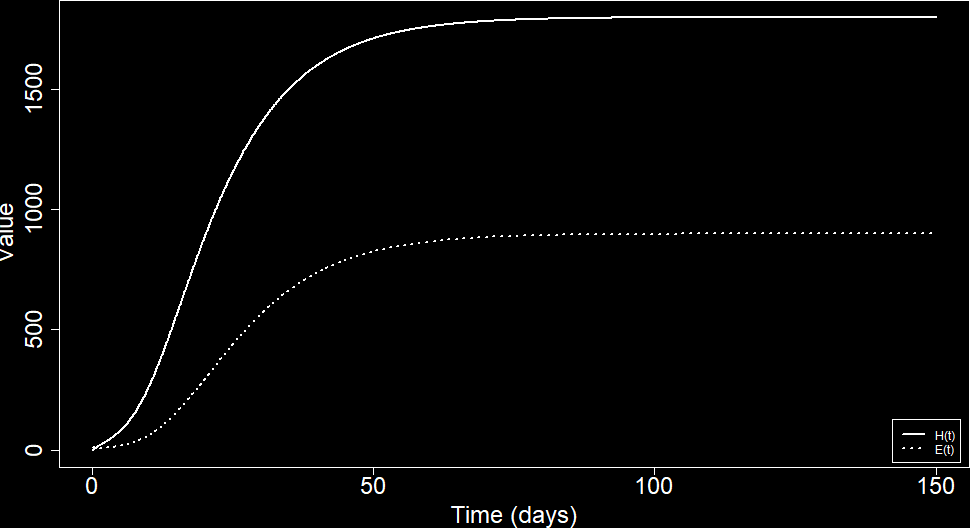
\includegraphics[width=\textwidth]{../FIGS/Capasso_ETP_1}
  \end{center}
\end{frame}

\begin{frame}
  Let
  \begin{equation}
    \label{eq:R0_capasso}
    \R_0 = \frac{g'_+(0)c_H}{d_E\gamma_H}
  \end{equation}
  \begin{theorem}
    \begin{itemize}
      \item If $0<\R_0<1$, then \eqref{sys:capasso_EH} admits only the trivial equilibrium in the positive orthant, which is GAS
      \item If $\R_0>1$, then two EP exist: $(0,0)$, which is unstable, and $z^\star=(E^\star,H^\star)$ with $E^\star,H^\star>0$, GAS in $\IR_+^2\setminus\{0,0\}$
    \end{itemize}
  \end{theorem}
\end{frame}

\begin{frame}[fragile]{Computing $\R_0$}
  With the chosen $g$, we have
  \[
    g'(E) = 
    \frac{N \beta pg_{half} g_{max}}
    {(g_{half}+E)^2}
  \]
  whence
  \[
    g_+'(0)=\frac{N \beta pg_{max}}
    {g_{half}}
  \]
  and thus
  \begin{equation}
    \R_0 = \frac{N \beta pg_{max}}
    {g_{half}}\;\frac{c_H}{d_E\gamma_H}
  \end{equation}
\begin{lstlisting}
R0 = function(params) {
  with(as.list(params), {
    R0 = N*beta*p*g_max*c_H / (g_half*d_E*gamma_H)
    return(R0)
  })
}  
\end{lstlisting}
\end{frame}


\begin{frame}{Showing things dynamically using Shiny}
  Shiny is an \code{R} library (made by RStudio) to easily make interactive displays
  \vfill
  See some documentation \href{https://shiny.rstudio.com/}{here}
  \vfill
  Some examples \href{https://shiny.rstudio.com/gallery/}{here} and \href{https://github.com/rstudio/shiny-examples}{here}
  \vfill
  Create a subdirectory with the name of your app and a file called \code{app.R} in there
\end{frame}


\begin{frame}{Structure of a Shiny app}
  Need to use library \code{shiny}
  \vfill
  Define two elements
  \begin{itemize}
    \item \code{ui}, which sets up the user interface
    \item \code{server}, which handles the computations, generation of figures, etc.
  \end{itemize}
  \vfill
  I explain different elements as we progress. See the code in the \code{CODE} folder and \code{Capasso\_simpleETP\_shiny} subdirectory
\end{frame}


\begin{frame}[fragile]{The \code{ui} part}
Here, we use \code{fluidPage} to create the UI. There are other functions: \code{fillPage}, \code{fixedPage}, \code{flowLayout}, \code{navbarPage}, \code{sidebarLayout}, \code{splitLayout} and \code{verticalLayout}
\vfill
\begin{lstlisting}
# Define UI
ui <- fluidPage(
)  
\end{lstlisting}
\vfill
We now fill this function
\end{frame}

\begin{frame}[fragile]{A title and some sliders}
\begin{lstlisting}
# Application title
titlePanel("Simple ETP model of Capasso"),
# Sidebar with slider inputs for some parameters
sidebarLayout(
    sidebarPanel(
      sliderInput("inv_gamma_H",
                  "Average infectious period (days):",
                  min = 0,
                  max = 30,
                  value = 10),
      sliderInput("c_H",
                  "Flow from humans:",
                  min = 0,
                  max = 2,
                  value = 0.1),
\end{lstlisting}
\vfill
Plus other sliders for all other parameters
\end{frame}

\begin{frame}[fragile]{Note the little trick...}
\begin{lstlisting}
sliderInput("inv_gamma_H",
"Average infectious period (days):",
min = 0,
max = 30,
value = 10),
\end{lstlisting}
\vfill
I want to give a user friendly version of the parameter value, using the number of days rather than the inverse, whereas the model uses the latter. So I prefix the variable name by \code{inv\_} and then process as follows in the \code{server} part
\begin{lstlisting}
params <- list()
for (param_name in names(input)) {
  if (grepl("inv_", param_name)) {
    new_param_name = gsubs("inv_", "", param_name)
    params[[new_param_name]] = 1/input[[param_name]]
  } else {
    params[[param_name]] = input[[param_name]]
  }
}
\end{lstlisting}
\end{frame}

\begin{frame}
  The simulation functions can be outside of \code{ui} or \code{server}, this makes the code neater
  \vfill
  These functions are the same as before (right hand side, g, h, R0), so they are not shown here
\end{frame}
    

\begin{frame}[fragile]{The \code{server} part}
\begin{lstlisting}
# Define server logic required to draw the result
server <- function(input, output) {
  ##
  ## Expression that generates the plot
  ##
  output$a_odePlot <- renderPlot({
    params <- list()
    params$N = 1000 # We could let this vary, we don't here..
    for (param_name in names(input)) {
      if (grepl("inv_", param_name)) {
        new_param_name = gsub("inv_", "", param_name)
        params[[new_param_name]] = 1/input[[param_name]]
      } else {
        params[[param_name]] = input[[param_name]]
      }
    }
    # Initial conditions and time span
    IC <- c(E = 10, H = 0)
    tspan <- seq(from = 0, to = params$tf, by = 0.1)  
\end{lstlisting}
\end{frame}
  

\begin{frame}[fragile]{The \code{server} part (continued)}
\begin{lstlisting}
    # Compute solution
    sol_ODE = ode(y = IC,
                  func = rhs_Capasso_ODE,
                  times = tspan,
                  parms = params)
    # Make the plot
    y_max = max(max(sol_ODE[,"H"]),sol_ODE[,"E"])
    plot(sol_ODE[,"time"], sol_ODE[,"H"],
          type = "l", lwd = 2,
          xlab = "Time (days)", ylab = "Value",
          ylim = c(0, y_max),
          main = sprintf("R_0=%1.2f", round(R0(params),2)))
    lines(sol_ODE[,"time"], sol_ODE[,"E"], 
          lwd = 2, lty = 3)
    legend("topleft", legend = c("H(t)", "E(t)"),
            lwd = c(2,2), lty = c(1,3), inset = 0.01)
  })
}
\end{lstlisting}
\end{frame}

\begin{frame}[fragile]{Finally, run the code}
\begin{lstlisting}
# Run the application 
shinyApp(ui = ui, server = server)
\end{lstlisting}
\end{frame}
  

\begin{frame}{Adding a periodic component}
  Assume $p$ in \eqref{eq:incidence_function_Capasso} takes the form 
  \begin{equation}
    p(t)=p(t+\omega)>0,\quad t\in\IR
  \end{equation}
  i.e., $p$ has period $\omega$. So we now consider the incidence
  \begin{equation}
    \label{eq:incidence_Capasso_periodic}
    g(t,E)=p(t)h(E)
  \end{equation}
  with $h$ having the properties prescribed earlier.
  Letting 
  \begin{equation}
    p_{min} := \min_{0\leq t\leq\omega}p(t),\quad
    p_{max} := \max_{0\leq t\leq\omega}p(t)
  \end{equation}
  then we require that 
  \begin{equation}
    \lim_{z\to\infty}\frac{g(z)}{z}<\frac{d_E\gamma_H}{c_Hp_{max}}
  \end{equation}
\end{frame}


\begin{frame}
  Let
  \begin{equation}
    \label{eq:R0_capasso_periodic}
    \R_0^{min} = \frac{c_Hp_{min}h'_+(0)}{d_E\gamma_H},\quad 
    \R_0^{max} = \frac{c_Hp_{max}h'_+(0)}{d_E\gamma_H}
  \end{equation}
  \begin{theorem}
    \begin{itemize}
      \item If $0<\R_0^{max}<1$, then \eqref{sys:capasso_EH} with incidence \eqref{eq:incidence_Capasso_periodic} always goes to extinction
      \item If $\R_0^{min}>1$, then a unique nontrivial periodic endemic state exists for \eqref{sys:capasso_EH} with incidence \eqref{eq:incidence_Capasso_periodic}
    \end{itemize}
  \end{theorem}
\end{frame}

\begin{frame}[fragile]{How to add periodicity in numerics?}
\begin{lstlisting}
p_t = function(t, params) {
  angle = 2*pi/params$p_period
  OUT = cos(angle*t) # Make the base cos wave
  OUT = OUT/2*(params$p_max-params$p_min) # Scale
  OUT = OUT-min(OUT)+params$p_min # Shift up
  return(OUT)
}   
g = function(E, params, t) {
  OUT = params$N * params$beta * p_t(t, params) * h(E,params)
  return(OUT)
}
R0 = function(params) {
  with(as.list(params), {
    R0 = list()
    R0$min = N*beta*p_min*g_max*c_H / (g_half*d_E*gamma_H)
    R0$max = N*beta*p_max*g_max*c_H / (g_half*d_E*gamma_H)
    return(R0)
  })
}  
\end{lstlisting}
\end{frame}


%%%%%%%%%%%%%%%%%%%%
%%%%%%%%%%%%%%%%%%%%
\subsection{The first schistosomiasis model of Woolhouse}
\begin{frame}{The model}
  Population of $H$ individuals using a body of water containing $N$ snails
  \vfill
  $I_H$ mean number of schistosomes per person and $i_S$ the proportion of patent infections in snails 
  (prevalence)
  \vfill
  \begin{subequations}
    \label{sys:Woolhouse}
    \begin{align}
      I_H' &= \alpha Ni_S-\gamma I_H \\
      i_S' &= \beta HI_H(1-i_S)-\mu_2 i_S
    \end{align}
  \end{subequations}
  \begin{itemize}
    \item $\alpha$ number of schistosomes produced per person per infected snail per unit time
    \item $1/\gamma$ average life expectancy of a schistosome
    \item $1/\mu_2$ average life expectancy of an infected snail
    \item $\beta$ transmission parameter
  \end{itemize}
\end{frame}


\begin{frame}[fragile]{Simulating -- The ODE}
\begin{lstlisting}
# Right hand side of the ODE
rhs_Woolhouse1_ODE = function(t, x, params) {
  with(as.list(c(x, params)), {
    dI_H = alpha*N*i_S-gamma*I_H
    di_S = beta*H*I_H*(1-i_S)-mu_2*i_S
    list(c(dI_H, di_S))
  })
}  
\end{lstlisting}
\end{frame}

\begin{frame}
  Let the basic reproductive rate for schistosomes be
  \begin{equation}
    \label{eq:R0_Woolhouse}
    \R_0 = \frac{\alpha N\beta H}{\gamma\mu_2}
  \end{equation}
  \vfill
  \eqref{sys:Woolhouse} has two EP
  \begin{itemize}
    \item $(I_H^\star,i_S^\star)=(0,0)$, LAS when $\R_0<1$ and unstable when $\R_0>1$
    \item $(I_H^\star,i_S^\star)=\left(\dfrac{\alpha N}{\gamma}-\dfrac{\mu_2}{\beta H},1-\dfrac{1}{\R_0}\right)$, which only ``exists'' when $\R_0>1$ (and is LAS then)
  \end{itemize}
\end{frame}

\begin{frame}[fragile]{Using $\R_0$ to set $\beta$}
\begin{lstlisting}
# Put parameters in a list
params = list()
params$H = 100        # Total human population
params$N = 1000       # Total population snails
params$alpha = 20     # Nb schistosomes/infected H/unit time
params$gamma = 1/1000 # Life expectancy schistosome
params$mu_2 = 1/70    # Life expectancy infected snail
# Set beta through R_0:
# R_0= alpha*N*beta*H/(gamma*mu_2),
# so, given R_0, 
# beta = R_0*gamma*mu_2/(alpha*N*H)
params$R_0 = 2.5     # Desired value of R_0
params$beta = params$R_0*params$gamma*params$mu_2 / 
  (params$alpha*params$N*params$H)
\end{lstlisting}
\end{frame}
    
    
  
\begin{frame}[fragile]{Helping these computations}
\begin{lstlisting}
R0_Woolhouse_ODE = function(params) {
  with(as.list(params), {
    R0 = alpha*N*beta*H/(gamma*mu_2)
    return(R0)
  })
}
EEP_Woolhouse_ODE = function(params) {
  with(as.list(params), {
    OUT = list()
    OUT$I_H = alpha*N/gamma-mu_2/(beta*H)
    OUT$i_S = 1-1/R0_Woolhouse_ODE(params)
    return(OUT)
  })
}  
\end{lstlisting}
\end{frame}

%%%%%%%%%%%%%%%%%%%%
%%%%%%%%%%%%%%%%%%%%
\subsection{The third schistosomiasis model of Woolhouse -- Heterogeneous contacts}
\begin{frame}{Heterogeneities in contact rates}
  $I_{i}$ the number of schistosomes in person $i=1,\ldots,H$ and $i_{Sj}$ the proportion of patent infected snails in site $j=1,\ldots,L$ ($L$ sites each supporting $N$ snails)
  \vfill
  \begin{center}
    \def\vertskip{*2}
    \def\horzskip{*1.5}
    \begin{tikzpicture}[scale=1, transform shape]
      \node [circle, fill=gray!10, text=black] at (-1\horzskip,0\vertskip) (site1) {$i_{S1}$};
      \node [circle, fill=gray!10, text=black] at (1\horzskip,0\vertskip) (site2) {$i_{S2}$};
      \node [circle, fill=gray!10, text=black] at (-1\horzskip,1\vertskip) (indiv1) {$I_1$};
      \node [circle, fill=gray!10, text=black] at (0\horzskip,1\vertskip) (indiv2) {$I_2$};
      \node [circle, fill=gray!10, text=black] at (1\horzskip,1\vertskip) (indiv3) {$I_3$};
      %% Flows between
      \path [line, very thick] (indiv1) to node [midway, below] (TextNode) {} (site1);
      \path [line, very thick] (indiv2) to node [near end, above] (TextNode) {} (site1);
      \path [line, very thick] (indiv2) to node [midway, below] (TextNode) {} (site2);
      \path [line, very thick] (indiv3) to node [midway, above] (TextNode) {} (site2);
      % Text
      \node [color=red] at (-2\horzskip,1\vertskip) {Individuals};
      \node [color=red] at (-2\horzskip,0\vertskip) {Sites};
    \end{tikzpicture}    
  \end{center}  
\end{frame}

\begin{frame}
  $I_{i}$ the number of schistosomes in person $i=1,\ldots,H$ and $i_{Sj}$ the proportion of patent infected snails in site $j=1,\ldots,L$ ($L$ sites each supporting $N$ snails)
  \begin{subequations}
    \label{sys:Woolhouse_3}
    \begin{align}
      I_{i}' &= \alpha\left(\sum_j \eta_{ij}Ni_{Sj}\right)-\gamma I_{i} \\
      i_{Sj}' &= \beta\left(\sum_i \eta_{ij}I_i\right)(1-i_{Sj})-\mu_2 i_{Sj}
    \end{align}
  \end{subequations}
  \vfill
  $\eta_{ij}$ rate of water contact by individual $i$ at site $j$
  \vfill  
\end{frame}


\begin{frame}{How to deal with large systems}
A system like \eqref{sys:Woolhouse_3} is a \textbf{large system} of ODE, as there are $H+L$ differential equations, with that number potentially large
\vfill
Large systems of this type (very few different types of equations) are quite simple numerically but require some organisation\dots 
\vfill
Rather than name the state variables, it is better to use the vector \code{x} with indices for the different types of variables
\end{frame}

\begin{frame}[fragile]{Indexing positions}
\begin{lstlisting}
params = list()
params$H = 100        # Total human population
params$L = 5          # Number of sites  
\end{lstlisting}
Then if we define
\begin{lstlisting}
params$idx_I_H = 1:params$H
params$idx_i_S = (params$H+1):(params$H+params$L)  
\end{lstlisting}
in the ODE, we will be able to use something like
\begin{lstlisting}
I_H = x[params$idx_I_H]
i_S = x[params$idx_i_S]
\end{lstlisting}
\end{frame}

\begin{frame}{Computing the incidence}
Here again, easy to do (and computationally efficacious) provided you are careful
\vfill
$K=[\eta_{ij}]$ is an $H\times L$ matrix. Denote $I_H=(I_{1},\ldots,I_{H})^T$ and $i_S=(i_{S1},\ldots,i_{SL})^T$
\vfill
Then
\[
  \sum_j \eta_{ij}Ni_{Sj} = N\sum_j \eta_{ij}i_{Sj}
  =K i_S
\]
and
\[
  \sum_i \eta_{ij}I_i = I_H^TK
\]
\end{frame}


% %%%%%%%%%%%%%%%%%%%%
% %%%%%%%%%%%%%%%%%%%%
% \subsection{Spatial aspects -- Cholera in Haiti}
% \begin{frame}{Spatial aspects -- Cholera in Haiti}
%   Tuite, Tien, Eisenberg, Earn, Ma \& Fisman.
%   \href{https://doi.org/10.7326/0003-4819-154-9-201105030-00334}{Cholera Epidemic in Haiti, 2010: Using a Transmission Model to Explain Spatial Spread of Disease and Identify Optimal Control Interventions}. \emph{Annals of Internal Medicine} \textbf{154}(9) (2011)
% \end{frame}

% \begin{frame}
%   \begin{center}
%     \def\vertskip{*1}
%     \def\horzskip{*4.5}
%     \begin{tikzpicture}[scale=0.9, transform shape]
%       \node [rectangle, fill=gray!10, text=black] at (0\horzskip,1.5\vertskip) (S_p) {$s_p$};
%       \node [rectangle, fill=gray!10, text=black] at (1\horzskip,1.5\vertskip) (I_p) {$i_p$};
%       \node [rectangle, fill=gray!10, text=black] at (2\horzskip,1.5\vertskip) (R_p) {$r_p$};
%       \node [circle, fill=gray!10, text=black] at (0.5\horzskip,4\vertskip) (W_p) {$W_p$};
%       \node [circle, fill=black, color=red, text=white] at (0.5\horzskip,1.5\vertskip) (lambda_p) {$\lambda_ps_p$};
%       \node [rectangle, fill=gray!10, text=black] at (0\horzskip,-1.5\vertskip) (S_q) {$s_q$};
%       \node [rectangle, fill=gray!10, text=black] at (1\horzskip,-1.5\vertskip) (I_q) {$i_q$};
%       \node [rectangle, fill=gray!10, text=black] at (2\horzskip,-1.5\vertskip) (R_q) {$r_q$};
%       \node [circle, fill=gray!10, text=black] at (0.5\horzskip,-4\vertskip) (W_q) {$W_q$};
%       %% Boxes
%       \path [line, rounded corners, thin] (-0.2\horzskip,0.8\vertskip) -- (-0.2\horzskip,4.75\vertskip) -- (2.2\horzskip,4.75\vertskip) -- (2.2\horzskip,0.8\vertskip) -- cycle;
%       \path [line, rounded corners, thin] (-0.2\horzskip,-0.8\vertskip) -- (-0.2\horzskip,-4.75\vertskip) -- (2.2\horzskip,-4.75\vertskip) -- (2.2\horzskip,-0.8\vertskip) -- cycle;
%       %% Flows in p
%       \draw [very thick, color=yellow] (S_p) -- (lambda_p);
%       \path [line, very thick] (lambda_p) to node [midway, above] (TextNode) {} (I_p);
%       \path [line, very thick] (I_p) to node [midway, above] (TextNode) {$\gamma i_p$} (R_p);
%       \path [line, very thick, dashed] (I_p) to node [midway, above] (TextNode) {$\xi i_p$} (W_p);
%       \path [line, very thick, dashed] (W_p) to node [midway, left] (TextNode) {$\beta_WW_p$} (lambda_p);
%       \path [line, very thick] (W_p) to node [midway, above] (TextNode) {$\xi W_p$} (0.1\horzskip,4\vertskip);
%       %% Flows in q
%       \path [line, very thick] (S_q) to node [midway, above] (TextNode) {$\lambda_qs_q$} (I_q);
%       \path [line, very thick] (I_q) to node [midway, above] (TextNode) {$\gamma i_q$} (R_q);
%       \path [line, very thick, dashed] (I_q) to node [midway, above] (TextNode) {$\xi i_q$} (W_q);
%       \path [line, very thick] (W_q) to node [midway, above] (TextNode) {$\xi W_q$} (0.1\horzskip,-4\vertskip);
%       %% lambda_p
%       \path [line, very thick, dashed] (I_q) to node [midway, left] (TextNode) {$\frac{\kappa P_pP_q}{d^n}$} (lambda_p);
%       \path [line, very thick, dashed, bend right=50] (I_p) to node [midway, below] (TextNode) {$\beta_Ii_p$} (lambda_p);
%       %% Distance between patches
%       \draw [line,very thick] (1.5\horzskip,0.8\vertskip) -- (1.5\horzskip,-0.8\vertskip);
%       \draw [line,very thick] (1.5\horzskip,-0.8\vertskip) -- (1.5\horzskip,0.8\vertskip);
%       \node [color=yellow, text width=3cm] at (1.85\horzskip,0\vertskip) {Distance between regions (d)};
%     \end{tikzpicture}    
%   \end{center}  
% \end{frame}

% %\maxFrameImage{../FIGS/Tuite_etal_cholera_model.png}

% \begin{frame}
%   \textbf{Metapopulation} model with \textbf{implicit} movement
%   \begin{subequations}
%     \begin{align}
%       s_p' &= \mu-\lambda_ps_p-\mu s_p \\
%       i_p' &= -\gamma i_p+\lambda_p s_p-\mu i_p \\
%       r_p' &= \gamma r_p-\mu r_p \\
%       w_p' &= \xi(i_p-w_p)
%     \end{align}
%     with force of infection
%     \begin{equation}
%       \lambda_p = \beta_{i_p}i_p+\beta_{W_p}w_p+\sum_{q=1}^{10}\theta_{pq}i_q
%     \end{equation}
%   \end{subequations}
%   \vfill
%   Influence of infection prevalence in $q$ on incidence in $p$ is gravity-type
%   \[
%     \theta_{pq}=\kappa\frac{P_pP_q}{d^n}
%   \]
% \end{frame}



\end{document}